\documentclass[a4paper,12pt,twoside]{article}
\usepackage[ngerman]{babel}
\usepackage[T1]{fontenc}
\usepackage[utf8]{inputenc}
\usepackage{fullpage}
\usepackage[table]{xcolor}
\usepackage{multirow}
\usepackage{graphicx}
\usepackage{caption}
\usepackage{subcaption}
\usepackage{wasysym}
\usepackage{geometry}
\usepackage[locale=DE]{siunitx}
\usepackage{eurosym}
\usepackage{placeins}
\usepackage{pdfpages}

\DeclareSIUnit{\EUR}{\text{\euro}}

\renewcommand\thesubfigure{\arabic{subfigure}}

\newcommand{\graybox}[1]{\colorbox{lightgray}{{\vrule height 10pt depth 0pt width 0pt}\hspace{#1}}}

\geometry{
  includehead,
  includefoot,
  top=1cm,
  headsep=.8cm,
  bottom=1cm,
  footskip=1cm,
  left=1.5cm,
  right=1.5cm,
  %showframe
}

\begin{document}
%\pagestyle{empty}
\begin{center}
  
\includegraphics[width=\textwidth]{Briefkopf.pdf} \\
  \vspace{2cm}
  {\Huge\textbf{Koordinatoren HowTo}} \vspace{1cm} \\
  {\large Uni-Sommerfest 2016}
\end{center}
\vfill
\begin{center}
  \begin{tabular}{p{2cm}p{4cm}cccp{1.1cm}p{2cm}p{1cm}}
    & & \multicolumn{2}{c}{Offen} \\
    \multirow{-2}{*}{\textbf{Theke}} & \multirow{-2}{*}{Angebot} & von & bis & \multirow{-2}{*}{\parbox{1cm}{Zapf\-schluss}} & \multirow{-2}{*}{\parbox{1cm}{Aufbau ab}} & \multirow{-2}{*}{Betreiber} & \multirow{-2}{*}{\parbox{1cm}{Liefer\-zone}} \\ \hline \hline
    Südhof & Bier, Cider, Non-Alk, Longdrinks & 19:00 & 4:30 & 4:00 & 14:00 & GAF & L1 \\ \hline
    Südhof (klein) & Bier, Cider, Non-Alk & 19:00 & 4:30 & 4:00 & 14:00 & Eva & L3 \\ \hline
    Südhof (Cocktail) & Cocktails & 19:00 & 4:30 & -- & 14:00 & TUM & L1 \\ \hline
    Lichthof & Bier, Cider, Non-Alk, Longdrinks & 19:00 & 4:40 & 4:10 & 14:00 & Computer\-linguistik & L2 \\ \hline
    Nordhof & Bier, Cider, Non-Alk & 19:00 & 3:30 & 3:00 & 14:00 & Biologie & L4 \\ \hline
    Halle Nord & Bier, Cider, Non-Alk, Longdrinks & 19:00 & 4:50 & 4:20 & 14:00 & Statistik & L5 \\ \hline
    Cafeteria & Non-Alk, Longdrinks & 19:00 & 4:50 & -- & 15:00 & Jura & L4 \\ \hline % Musik ab 21:00
    AdaHa & Bier, Cider, Non-Alk, Longdrinks & 19:00 & 4:50 & 4:20 & 14:00 & Chemie & L8 \\ \hline
    Bierprobe Haußmann & Bierspezialitäten & 19:00 & 3:30 & 3:00 & 15:00 & Haußmann & L6 \\ \\
                        & & \multicolumn{2}{c}{Offen} \\
    \multirow{-2}{*}{\textbf{Markenverkauf}} & & von & bis & & \multirow{-2}{*}{\parbox{1cm}{Aufbau ab}} \\ \hline \hline
    %\textbf{Markenverkauf} \\ \hline \hline
    Eulenbrunnen & & 19:00 & 4:30 & & 15:00 \\
    Lichthof & & 19:00 & 4:40 & & 15:00 \\
    Nordhof & & 19:00 & 5:10 & & 15:00 \\
    Eingang & & 18:00 & 1:30 & & 15:00
  \end{tabular}
\end{center}

Die Zentrale ist unter \textbf{089/2180-17960} erreichbar. Ruft dort im Notfall an: Sanitäter oder Security wird benötigt, Feuer, o.ä.

Auch wenn ihr dringend etwas von den Getränkekoordinatoren braucht, könnt ihr euch dort melden und die Zentrale funkt uns dann an.

% ---
\section{Vor dem Fest}
\subsection{Getränke und Equipment}
\begin{itemize}
  \item Auf Paletten an der zugeordneten Lieferzone:
    \begin{itemize}
      \item Bier- und Ciderfässer
      \item Non-Alk und Bier in Kästen
      \item Hard-Alk in Kartons (ab ca. 15:00 Uhr)
      \item Zapfanlagen
      \item Becher in Plastikkisten (0,3l \& 0,5l)
      \item Kühlschränke

        Bänder um die Kühlschränke \textbf{unbedingt} aufheben!
      \item Biertischgarnituren
      \item Eis in Gefriertruhen oder Thermoboxen
    \end{itemize}
  \item CO$_2$-Flaschen sind im Müllgang. Vorsichtig tragen und gegen Umfallen schützen!
  \item Equipment abholen:
    \begin{itemize}
      \item Thekenkisten mit Klebeband, Zangen, Kabelbindern usw.\ sind im Lager (Raum A120) % TODO Raum richtig?
      \item Helferkisten mit T-Shirts, Bändern, Marken usw.\ sind in der Helferzentrale (Senatssaal Raum E106 \& E110)
    \end{itemize}
  \item Pavillons sind bereits aufgebaut
  \item Feuerlöscher stehen bereit
\end{itemize}
% ---
\subsection{Thekenaufbau}
Siehe Abbildungen \ref{theke2d} und \ref{theke3d}.
\begin{figure}[h]
  \centering
  \begin{subfigure}[t]{0.45\textwidth}
    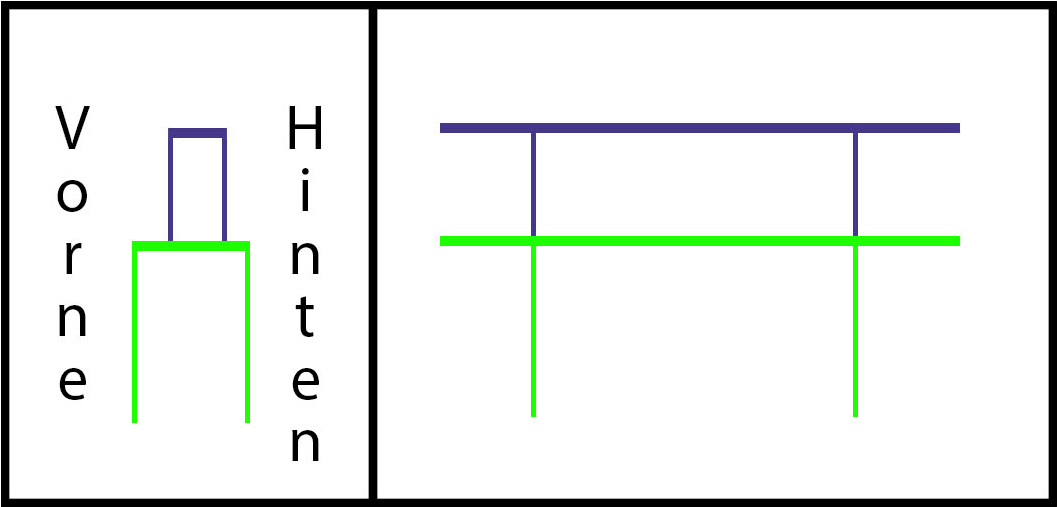
\includegraphics[width=\textwidth]{2d_1.png}
    \caption{Einen Tisch aufstellen und eine aufgeklappte Bank darauf stellen.}
  \end{subfigure}
  \hfill
  \begin{subfigure}[t]{0.45\textwidth}
    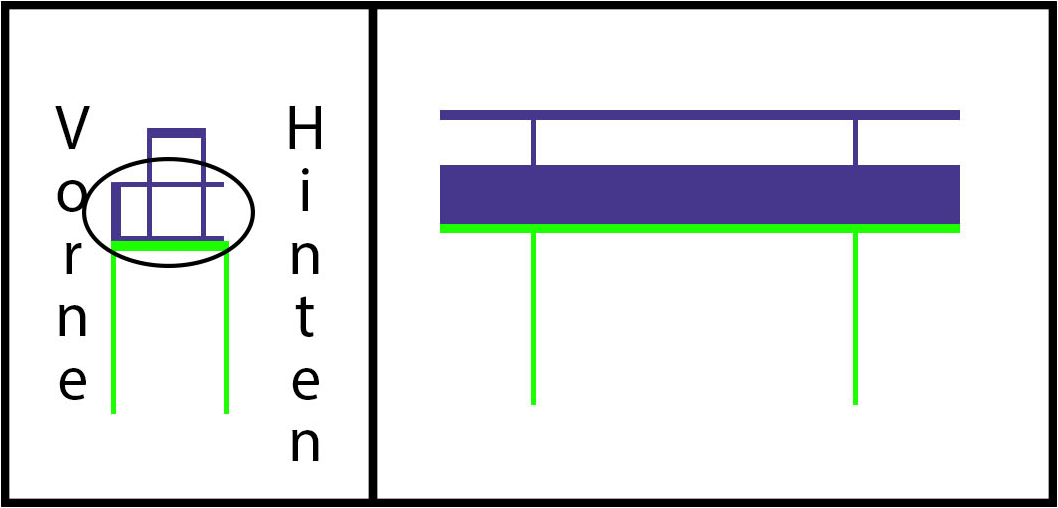
\includegraphics[width=\textwidth]{2d_2.png}
    \caption{Eine Bank aufklappen, aber die diagonalen Arretierungen eingeklappt lassen. Die Bank senkrecht zum Tisch hinlegen und alle drei Teile mit Kabelbindern befestigen, aber noch nicht ganz festzurren.}
  \end{subfigure}
  \centering
  \begin{subfigure}[t]{0.45\textwidth}
    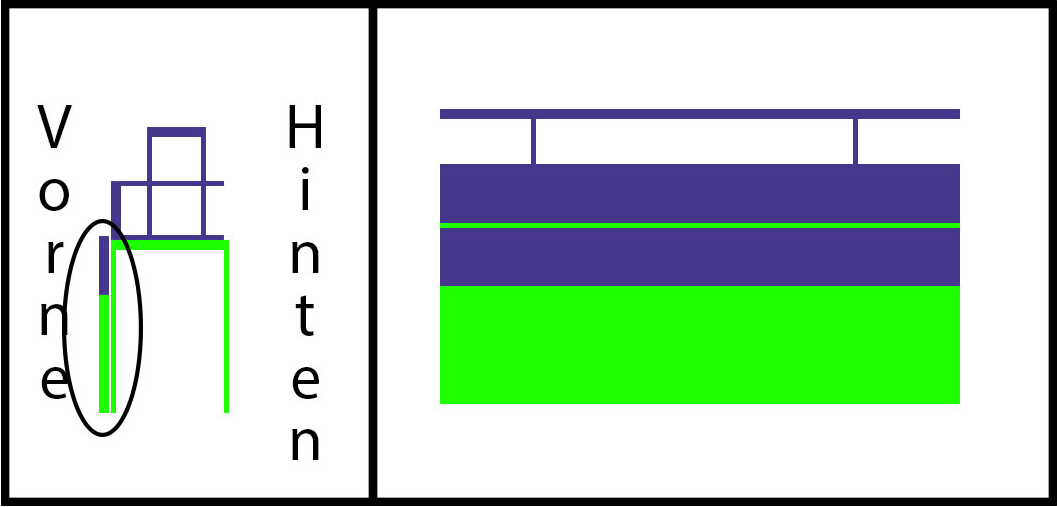
\includegraphics[width=\textwidth]{2d_3.png}
    \caption{Die Vorderseite mit 1 Tisch und 2 Bänken, oder 3 Bänken verkleiden und mit Kabelbindern verbinden (die Beine jeweils eingeklappt lassen, sonst stehen sie innen über).}
  \end{subfigure}
  \hfill
  \begin{subfigure}[t]{0.45\textwidth}
    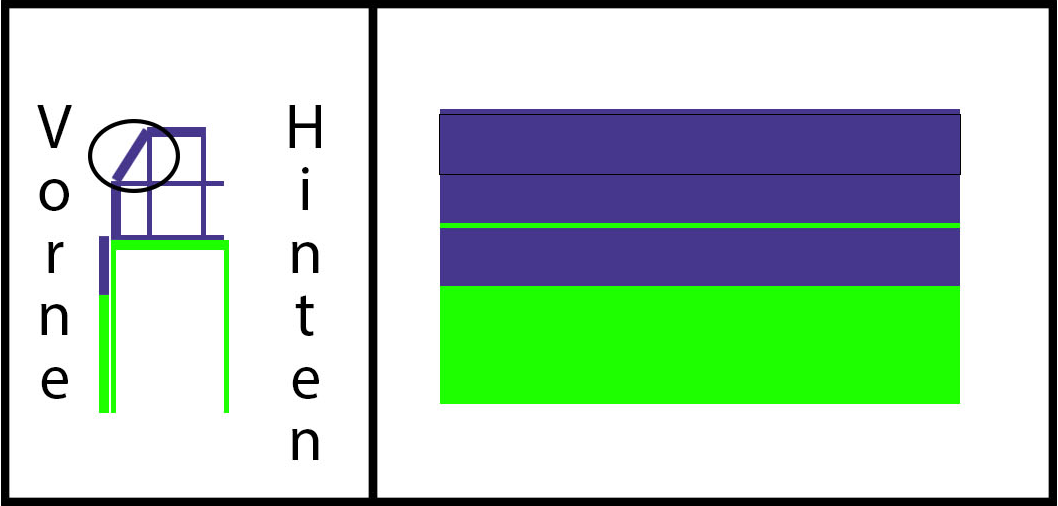
\includegraphics[width=\textwidth]{2d_4.png}
    \caption{Eine Bank (auch ohne Beine) schräg zwischen der liegenden und der stehenden Bank einspannen und mit Kabelbindern festzurren.}
  \end{subfigure}
  \caption{Aufbau einer Theke aus 2 Tischen (grün) und 4 Bänken (blau) oder 1 Tisch und 6 Bänken.}
  \label{theke2d}
\end{figure}

\begin{figure}[h]
  \begin{subfigure}[t]{0.45\textwidth}
    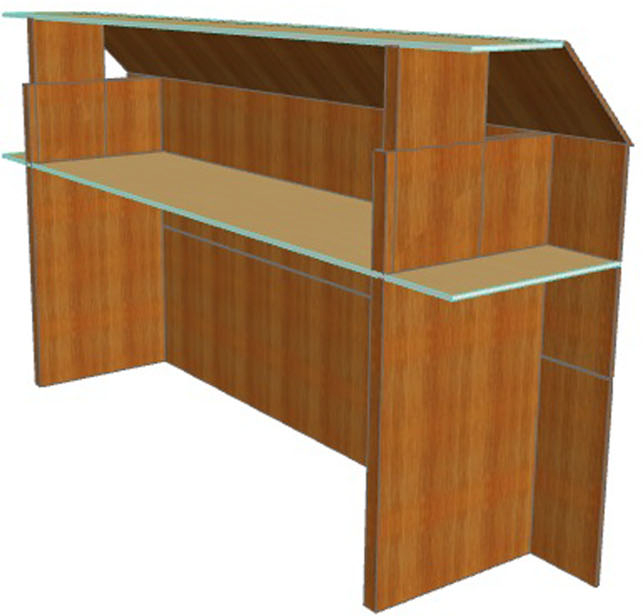
\includegraphics[width=\textwidth]{3d_hinten.png}
    \caption{Ansicht von hinten.}
  \end{subfigure}
  \begin{subfigure}[t]{0.45\textwidth}
    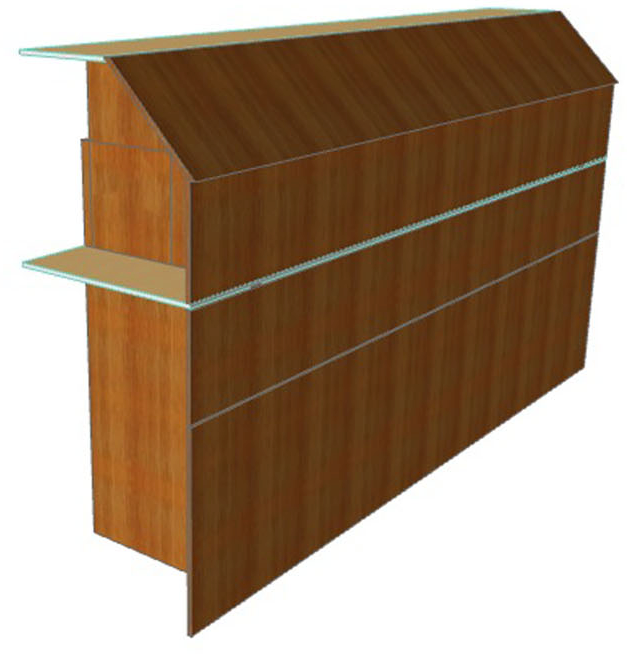
\includegraphics[width=\textwidth]{3d_vorne.png}
    \caption{Ansicht von vorne.}
  \end{subfigure}
  \caption{So sollte eure Theke mehr oder weniger aussehen.}
  \label{theke3d}
\end{figure}

% ---
\subsection{Schilder}
\begin{itemize}
  \item Geklebt werden darf auf \textbf{nur} auf unsere Aufbauten und Kühlschränke
  \item Alles nur mit Kreppband kleben und \textbf{niemals} auf verputzte oder gestrichene Wände!
  \item Aufgehängt werden müssen
    \begin{itemize}
      \item Thekenbeschilderung: Getränkeangebot, laminiert A4/A3 auf die Thekenelemente
      \item Jugendschutzgesetze
    \end{itemize}
  \item Eigene Banner der Fachschaft o.ä.\ müssen mit uns \textbf{rechtzeitig} vorher abgesprochen werden (u.A.\ wegen des Brandschutzzertifikats)

    Ohne Absprache mitgebrachte Banner können \textbf{nicht} aufgehängt werden!
\end{itemize}
% ---
\subsection{Deadlines}
\begin{itemize}
  \item Zapfanlagen fertig bis \textbf{16:30} für Getränkerundgang und Abnahme der Schankanlagen
  \item Thekenfronten fertig bis \textbf{16:30} für KVR-Rundgang um \textbf{17:00}
  \item Theke innen fertig aufbauen und betriebsfertig machen!

    Alle Getränke zählen und in die angehängte Liste (\emph{Vorher}) eintragen. Nach dem Fest zusammen mit der zweiten ausgefüllten Liste (\emph{Nachher}) einem Getränkeorga geben (Felix, Markus oder Christoph).
  \item \large{Fest beginnt um \textbf{19:00}!}
\end{itemize}

% ---
\section{Während des Fests}
\subsection{Markensystem}
\begin{itemize}
  \item Wert einer Marke: {\large\SI{1.25}{\EUR}}
  \item Wertmarken sind \textbf{grün}, Helfermarken sind \textbf{orange} und \textbf{quadratischer} als die Wertmarken.
  \item Getränkepreise:

    \begin{tabular}{lll}
      Non-Alk & 1 Marke & + 1 Marke Pfand \\
      Bier, Cider, Energydrink & 2 Marken & + 1 Marke Pfand \\
      Longdrinks & 3 Marken & + 1 Marke Pfand \\
      Cocktails & 4 Marken & + 1 Marke Pfand
    \end{tabular}
  \item Wenn 1 Marke Pfand bezahlt wurde, \textbf{muss} zusammen mit dem Becher (bzw. Flasche) \textbf{1 Pfandmarke} (pink) ausgegeben werden.
  \item \textbf{Alle} Getränke werden mit Marken bezahlt. Wer Freigetränke bekommt (Helfer, Orgas, Musiker etc.), hat von uns genug Helfermarken bekommen. Es gehen \textbf{keine} Getränke ohne Bezahlung durch Wert- oder Helfermarken über die Theke!
  \item An der Theke gibt es \textbf{kein} Bargeld!
    \begin{itemize}
      \item Getränke können nur mit Marken bezahlt werden, \textbf{nicht} in bar.
      \item Marken können an der Theke \textbf{nicht} wieder in Bargeld umgetauscht werden.
      \item Geld zurück, z.B.\ Pfand, gibt es \textbf{nur} am Markenverkauf!
    \end{itemize}
  \item Alle Marken werden \textbf{zerrissen und entsorgt}, sobald sie als Bezahlung angenommen und gezählt wurden!
\end{itemize}
% ---
\subsection{Helfergetränke}
\begin{itemize}
  \item Es gibt eigene Helfermarken (orange).
  \item Alle, die mit Helfermarken zahlen, geben \textbf{keine} Wertmarke für Pfand ab und bekommen auch \textbf{keine} Pfandmarke.
  \item Für hinter der Theke verbrauchte Getränke müssen keine Helfermarken gezahlt werden. Bitte tragt diese in die dafür vorgesehene Strichliste ein.
\end{itemize}
% ---
\subsection{Ein Gast kommt an die Theke}
\begin{enumerate}
  \item Der Gast hat noch keinen Becher:
    \begin{itemize}
      \item Er/Sie bezahlt den \textbf{Getränkepreis + 1 Marke Pfand}.
      \item Er/Sie bekommt dafür das Getränk \textbf{+ 1 Pfandmarke (pink)}.
    \end{itemize}
  \item Der Gast hat schon einen Becher:
    \begin{itemize}
      \item Er/Sie gibt den Becher ab und bezahlt das Getränk -- \textbf{keine} Marke extra für Pfand.
      \item Er/Sie bekommt ein neues Getränk und \textbf{keine} Pfandmarke -- er/sie hat ja von vorher noch eine.
    \end{itemize}
  \item Der Gast ist ein Helfer/Koordinator/Orga:
    \begin{itemize}
      \item Er/Sie gibt die passende Menge Helfermarken ab -- \textbf{keine} Marke extra für Pfand (egal ob ein Becher zurückgegeben wurde oder nicht).
      \item Er/Sie bekommt dafür das Getränk und \textbf{keine} Pfandmarke.
    \end{itemize}
\end{enumerate}
% ---
\subsection{Getränke}
\subsubsection{Bier und Cider}
\begin{itemize}
  \item Bier (Augustiner Hell) in \SI{50}{\litre}-Fässern
  \item Cider (Strongbow) in \SI{30}{\litre}-Fässern
  \item Bier, Radler und Cider werden in \SI{0.5}{\litre}-Bechern ausgeschenkt.
  \item Nach Zapfschluss wird kein neues Fass Bier mehr angebrochen. Stattdessen wird Bier aus den Kästen \textbf{in Becher umgefüllt}. Glasflaschen werden \textbf{nicht} ausgegeben.
\end{itemize}
% ---
\subsubsection{Crown's Energy}
\begin{itemize}
  \item Crown's Energy wird \textbf{nicht} in Dosen ausgegeben, sondern mit etwas Eis im Becher verkauft.
  \item Kostet \textbf{2} Marken, obwohl es Non-Alk ist.
  \item Die zurückgegebenen Dosen kommen in gesonderte Säcke (von Leckerland).
\end{itemize}
% ---
\subsubsection{Non-Alk}
\begin{itemize}
  \item Es gibt Cola, Spezi, Apfelschorle, Zitronenlimo und Wasser (in zwei Sorten: wenig und viel Kohlensäure).
  \item Non-Alk wird \textbf{ohne} Becher in der PET-Flasche verkauft. Wie bei allen Getränken kommt eine Marke für den \textbf{Pfand} dazu und eine Pfandmarke wird ausgegeben.
  \item Es gibt Cola und Wasser in zwei Versionen:
    \begin{itemize}
      \item \SI{0.5}{\litre}-Flasche von Aloisius-Quelle $\rightarrow$ wird als Non-Alk verkauft
      \item \SI{1}{\litre}-Flasche von Coca Cola bzw. Adelholzener $\rightarrow$ wird \textbf{nur} zum Mischen von Rum-Cola bzw.\ Prosecco Aperol verwendet
    \end{itemize}
\end{itemize}
% ---
\subsubsection{Longdrinks}
\begin{enumerate}
  \item ca.\ \SI{100}{\gram} \textbf{Eis} mit der dafür vorgesehenen Schaufel in einen frischen \SI{0.3}{\litre}-Becher
  \item den \textbf{Alkohol} mit dem Dosierer in der richtigen Menge einschenken.
    
    Der Dosierer muss dafür im richtigen Winkel gehalten werden: Hals des Dosierers senkrecht, nicht die Flasche! Dann stoppt der Dosierer nach \SI{5}{\centi\litre}. Um erneut \SI{5}{\centi\litre} einzuschenken, muss die Flasche einmal aufgerichtet werden.
  \item mit \textbf{Non-Alk} auffüllen
  \item einen \textbf{Strohhalm} dazu
\end{enumerate}

\paragraph{Mischverhältnisse}
\begin{center}
  \begin{tabular}{llll}
    Longdrink & Alkohol & Non-Alk & Eis \\ \hline\hline
    Wodka-Orange &  \SI{5}{\centi\litre} Wodka & \SI{15}{\centi\litre} Orangensaft & $\sim$\SI{100}{\gram} \\ \hline
    Wodka-Lemon & \SI{5}{\centi\litre} Wodka & \SI{15}{\centi\litre} Bitter Lemon & $\sim$\SI{100}{\gram} \\ \hline
    Wodka-Energy & \SI{5}{\centi\litre} Wodka & \SI{15}{\centi\litre} Crown's Energy & $\sim$\SI{100}{\gram} \\ \hline
    Crown's Energy & -- & \SI{25}{\centi\litre} (Eine Dose Crown's Energy) & $\sim$\SI{100}{\gram} \\ \hline
    Rum-Cola & \SI{5}{\centi\litre} Rum & \SI{15}{\centi\litre} Coca Cola & $\sim$\SI{100}{\gram} \\ \hline
    Malibu-Kirsch & \SI{10}{\centi\litre} Malibu & 10cl Kirschsaft & $\sim$\SI{100}{\gram} \\ \hline
    Gin-Tonic & \SI{5}{\centi\litre} Gin & \SI{15}{\centi\litre} Tonic Water & $\sim$\SI{100}{\gram} \\ \hline
    Prosecco Aperol & \SI{5}{\centi\litre} Aperol \& \SI{10}{\centi\litre} Proseco & \SI{3}{\centi\litre} Mineralwasser & $\sim$\SI{100}{\gram} \\ \hline
    Hugo & Fertig ca. \SI{20}{\centi\litre} & $\sim$3 Minzblätter
  \end{tabular}
\end{center}

\paragraph{Alkoholsorten}
\begin{itemize}
  \item Wodka: Smirnoff Red Label (\SI{1}{\litre}-Flasche)
  \item Rum: Havanna Club 3 Jahre (\SI{1}{\litre}-Flasche)
  \item Malibu (\SI{1}{\litre}-Flasche)
  \item Gin: Gordon's Dry Gin (\SI{1}{\litre}-Flasche)
  \item Prosecco (\SI{0.7}{\litre}-Flasche)
  \item Aperol (\SI{1}{\litre}-Flasche)
\end{itemize}

% ---
\subsubsection{Cocktails}
\begin{table}[h!]
  \begin{subtable}[t]{0.3\textwidth}
    \vspace{0pt}
    \begin{tabular}{|rl|} \hline
      \multicolumn{2}{|l|}{\textbf{Zombie}} \\
      \SI{2}{\centi\litre} & weißer Rum \\
      \SI{2}{\centi\litre} & brauner Rum \\
      \SI{1}{\centi\litre} & Rum, 73\% \\
      \SI{1}{\centi\litre} & Apricot Brandy \\
      \SI{5}{\centi\litre} & Ananassaft \\
      \SI{2}{\centi\litre} & Limettensaft \\
      1 Scheibe & Orange \\
      1 Blatt & Minze \\ \hline
    \end{tabular}
  \end{subtable}
  ~
  \begin{subtable}[t]{0.3\textwidth}
    \vspace{0pt}
    \begin{tabular}{|rl|} \hline
      \multicolumn{2}{|l|}{\textbf{Touchdown}} \\
      \SI{4}{\centi\litre} & Wodka \\
      \SI{2}{\centi\litre} & Apricot Brandy \\
      \SI{6}{\centi\litre} & Maracujasaft \\
      \SI{2}{\centi\litre} & Orangensaft \\
      \SI{2}{\centi\litre} & Zitronensaft \\
      \SI{1}{\centi\litre} & Grenadinensirup \\ \hline
    \end{tabular}
  \end{subtable}
  ~
  \begin{subtable}[t]{0.3\textwidth}
    \vspace{0pt}
    \begin{tabular}{|rl|} \hline
      \multicolumn{2}{|l|}{\textbf{Sex on the Beach}} \\
      \SI{4}{\centi\litre} & Wodka \\
      \SI{2}{\centi\litre} & Peach Tree Likör \\
      \SI{2}{\centi\litre} & Zitronensaft \\
      \SI{4}{\centi\litre} & Orangensaft \\
      \SI{4}{\centi\litre} & Ananassaft \\
      \SI{1}{\centi\litre} & Grenadinensirup \\ \hline
    \end{tabular}
  \end{subtable}

  \vspace{1cm}
  \begin{subtable}[t]{0.3\textwidth}
    \vspace{0pt}
    \begin{tabular}{|rl|} \hline
      \multicolumn{2}{|l|}{\textbf{Jubiläumscocktail}} \\
      \SI{4}{\centi\litre} & brauner Rum \\
      \SI{2}{\centi\litre} & Apricot Brandy \\
      \SI{6}{\centi\litre} & Maracujasaft \\
      \SI{1}{\centi\litre} & Limettensaft \\
      \SI{1}{\centi\litre} & Grenadinensirup \\ \hline
    \end{tabular}
  \end{subtable}
  ~
  \begin{subtable}[t]{0.3\textwidth}
    \vspace{0pt}
    \begin{tabular}{|rl|} \hline
      \multicolumn{2}{|l|}{\textbf{Tequila Sunrise}} \\
      \SI{5}{\centi\litre} & Tequila \\
      \SI{10}{\centi\litre} & Orangensaft \\
      \SI{1}{\centi\litre} & Grenadinensirup \\ \hline
    \end{tabular}
  \end{subtable}
  ~
  \begin{subtable}[t]{0.3\textwidth}
    \vspace{0pt}
    \begin{tabular}{|rl|} \hline
      \multicolumn{2}{|l|}{\textbf{Mojito}} \\
      \SI{6}{\centi\litre} & weißer Rum \\
      \SI{12}{\centi\litre} & Mineralwasser \\
      \SI{0.5}{EL} & weißer Rohrzucker \\
      \num{0.5} & Limette \\ \hline
    \end{tabular}
  \end{subtable}
  
  \vspace{1cm}
  \begin{subtable}[t]{0.3\textwidth}
    \vspace{0pt}
    \begin{tabular}{|rl|} \hline
      \multicolumn{2}{|l|}{\textbf{Caipirinha}} \\
      \SI{10}{\centi\litre} & Cachaça \\
      \num{1} & Limette \\
      \SI{2}{EL} & brauner Rohrzucker \\
      Rest & Wasser \\ \hline
    \end{tabular}
  \end{subtable}
  ~
  \begin{subtable}[t]{0.3\textwidth}
    \vspace{0pt}
    \begin{tabular}{|rl|} \hline
      \multicolumn{2}{|l|}{\textbf{Non-Alk}} \\
      \SI{3}{\centi\litre} & Zitronensaft \\
      \num{1} & Limette \\
      \SI{1.5}{EL} & brauner Rohrzucker \\
      \SI{6}{\centi\litre} & Maracujasaft \\
      Rest & Wasser \\ \hline
    \end{tabular}
  \end{subtable}
  ~
\end{table}

% ---
\section{Nach dem Fest}
% ---
\subsection{Inventur}
Zählt bitte \textbf{alle} übrigen Getränke und tragt sie in die angehängte Liste (\emph{Nachher}) ein. Gebt die Mengen in \textbf{Kästen} (Non-Alk, Bier), \textbf{Fässern} (Bier, Cider) und \textbf{Kartons} (Schnaps, Prosecco etc.) an.

Gebt diese Liste zusammen mit der Liste mit den Getränken der Thekenhelfer einem der Getränkeorgas: Felix, Markus oder Christoph.
% ---
\subsection{Getränke}
\begin{itemize}
  \item Übrige, noch geschlossene, Schachteln mit Schnapsflaschen bitte nach Absprache mit einem Getränke-Orga verräumen.
  \item Offene Flaschen an andere, noch offene Theken bringen, falls möglich.
  \item Eis über dem nächsten Gulli ausleeren. Die \textbf{Styroporkisten} bitte nicht kaputtmachen, dafür zahlen wir Pfand!
\end{itemize}
% ---
\subsection{Paletten}
\begin{itemize}
  \item Biertischgarnituren: \begin{itemize}
      \item Je 20 Biertischgarnituren werden auf eine \textbf{große} Palette gestapelt.
      \item Pro Ebene liegt eine Garnitur (1 Tisch und 2 Bänke).
      \item \textbf{Alle} Tische und Bänke mit der Oberseite nach \textbf{unten}.
      \item Jeweils \textbf{Tische auf Bänke} und \textbf{Bänke auf Tische} stapeln, also immer abwechselnd.
      \item Danach sichern wir alles mit Palettenband. Ihr müsst also keine Spanngurte o.ä.\ verwenden.
    \end{itemize}
  \item Fässer und Kästen -- soweit möglich -- nach voll und leer getrennt auf Paletten.
  \item Becherkisten sortieren nach
    \begin{itemize}
      \item \SI{0.3}{\litre} oder \SI{0.5}{\litre}
      \item benutzt oder unbenutzt
    \end{itemize}
    Insgesamt also 4 Stapel auf getrennten Paletten!
  \item Alle kleinen Paletten bitte mit der \textbf{schmalen} Seite zum Weg, sodass sie direkt mit dem Stapler erreichbar sind.
  \item Alle großen Paletten mit Biertischgarnituren bitte mit der \textbf{breiten} Seite zum Weg.
\end{itemize}
% ---
\subsection{Equipment}
\begin{itemize}
  \item Jeweils 2 \textbf{Kühlschränke} auf eine kleine Palette und mit dem mitgelieferten Band sichern.
  \item \textbf{Zapfanlagen} in Kisten verpacken.
    
    Falls ohne Kiste geliefert, jeweils 4 Zapfen auf eine kleine Palette stellen.
  \item \textbf{CO$_2$-Flaschen} zurück in den Müllgang tragen. Vorsicht, nicht fallen lassen!
  \item \textbf{Müll} im Müllgang in die entsprechenden Mülltonnen entsorgen: Restmüll, Glasflaschen \textbf{ohne} Pfand (Schnaps u.ä.), Papier
  \item \textbf{Feuerlöscher} ins Möbellager bringen.
  \item \textbf{Pfandmarken} zurück in die Thekenkisten.
    
    \textbf{Thekenkisten und Helferkisten} wieder zusammenpacken und ins Lager (Raum A120) bringen.
  \item \textbf{Pavillons} stehen lassen.
\end{itemize}
% ---
\subsection{Heimgehen und ausschlafen \smiley}
Vielen Dank für eure Hilfe!

% ---
\section{Helfereinweisung}
Diese Einweisung sollte jeder, der an eurer Theke hilft, zu Schichtbeginn bekommen.
\subsection{Verkauf und Pfand}
\begin{itemize}
  \renewcommand{\labelitemi}{$\Box$}
  \item Es gibt kein Bargeld an der Theke und es kann nicht bar bezahlt werden. Es müssen Marken am Markenverkauf gekauft werden.
  \item Marken nach Annahme zählen und wenn passend zerreißen und wegschmeißen.
  \item Es wird \textbf{nicht} nachgeschenkt. Die Alkoholmenge ist mit dem Dosierer genau festgelegt: \SI{5}{\centi\litre} bei den Longdrinks mit Wodka, Gin und Rum bzw.\ \SI{10}{\centi\litre} bei Malibu-Kirsch.
  \item Non-Alk wird in der Plastikflasche ausgegeben, auch 1 Marke Pfand.
  \item Zu allen Getränkepreisen kommt 1 Marke Pfand dazu und es wird eine \textbf{Pfandmarke} ausgegeben!
    
    Wenn ein Becher zurückgegeben wurde, nur den Becher zurücknehmen, \textbf{keinen} Pfand verlangen und auch \textbf{keinen} Pfandbon ausgeben (der Gast hat ja noch seinen Pfandbon).
  \item Pfand können Gäste an der Theke nicht zurückbekommen, weder bar noch als Marken. Pfandrückgabe gibt es nur an der Markenausgabe.
  \item \textbf{Preisliste zeigen}
\end{itemize}
% ---
\subsection{T-Shirts}
\begin{itemize}
  \renewcommand{\labelitemi}{$\Box$}
  \item Helfer-T-Shirt hinter der Theke anhaben.
  \item Helfer-T-Shirt außerhalb der Schicht ausziehen!
  \item T-Shirt Farben: Helfer (grün), Koordinatoren (blau) und Organisatoren (lila bzw.\ grau für Pullis)
\end{itemize}
% ---
\subsection{Helfergetränke}
\begin{itemize}
  \renewcommand{\labelitemi}{$\Box$}
  \item Während der Schicht sind Helfergetränke kostenlos, davor und danach Marken benutzen. Diese bekommt man nur persönlich in der Helferzentrale.
  \item Helfergetränke für Helfer \textbf{unserer Theke} werden in einer Strichliste eingetragen.
  \item \textbf{Alle die Getränke kostenlos bekommen, haben Marken. Niemand bekommt Getränke einfach so.}
  \item Helfer zahlen keinen Pfand und bekommen auch keine Pfandmarke, zahlen also nur die passende Menge an Helfermarken: \textbf{Zeigen, wie Helfermarken aussehen}
\end{itemize}
% ---
\subsection{Mischen und Zapfen}
\begin{itemize}
  \renewcommand{\labelitemi}{$\Box$}
  \item \textbf{Zeigen, wie man Longdrink mischt und Bier und Cider zapft!}
  \item Auf den Boden gefallene Strohhalme etc. in den Müll
  \item Becher nie von oben anfassen. Nur frische Becher verwenden.
\end{itemize}
% ---
\subsection{Sicherheit}
\begin{itemize}
  \renewcommand{\labelitemi}{$\Box$}
  \item Bei Problemen (Schlägerei, pöbelnde Kunden, nicht bezahlte Getränke etc.) Koordinatoren holen, dann rufen sie Orgas/Securities. \textbf{Nicht} selber dazwischen gehen!
  \item \textbf{Fluchtwege zeigen!}
  \item Feuerlöscher stehen bereit: \textbf{Zeigen, wo hinter der Theke}.
    
    Bei Feuer: \textbf{Erst} Orgas verständigen bzw.\ Feuerwehr rufen, \textbf{dann} versuchen, das Feuer zu löschen:
    
    Stift aus dem Griff ziehen und Griff zusammendrücken. \textbf{Kurze} Sprühstöße mit dem Löscher
  \item Bei Verletzungen Erste Hilfe leisten und Sanis rufen (über Orgas oder Securities)
  \item \textbf{Niemand} außer Orgas (dunkelrote Shirts) und zur Theke gehörende Helfer dürfen hinter die Theke. Bei Zweifel fragen bzw.\ Koordinatoren rufen.
\end{itemize}
% ---
\subsection{Verpflegung und Helfermarken}
\begin{itemize}
  \item Essen gibt es in der Helferzentrale (E106)
  \item Helfermarkenmarken gibt es in der Helferzentrale -- sie werden nicht mehr von den Koordinatoren verteilt.
\end{itemize}

% ---
\section{Inventur}
\newcommand{\inputfield}[1][5cm]{\underline{\hspace{#1}}}

\newcommand{\inventurliste}[2]{
\cleardoublepage
{\large
\begin{center}
\begin{tabular}{|p{2cm}|lrll|l|}
  \multicolumn{5}{l}{Theke: \inputfield \quad #1} & \multicolumn{1}{r}{\textbf{#2}} \\ \hline
  \multirow{3}{*}{\parbox{2cm}{Bier/\quad Cider}}
  & Augustiner      & \SI{50}{\litre}             &      & Fass   & \inputfield \\
  & Strongbow       & \SI{30}{\litre}             &      & Fass   & \inputfield \\
  & Augustiner      & 20$\times$\SI{0.5}{\litre}  & Glas & Kasten & \inputfield \\
  \hline
  \multirow{7}{*}{Non-Alk}
  & Zitronenlimo    & 20$\times$\SI{0.5}{\litre}  & PET  & Kasten & \inputfield \\
  & Apfelschorle    & 20$\times$\SI{0.5}{\litre}  & PET  & Kasten & \inputfield \\
  & Cola-Mix        & 20$\times$\SI{0.5}{\litre}  & PET  & Kasten & \inputfield \\
  & Cola            & 20$\times$\SI{0.5}{\litre}  & PET  & Kasten & \inputfield \\
  & Orangenlimo     & 20$\times$\SI{0.5}{\litre}  & PET  & Kasten & \inputfield \\
  & Wasser medium   & 20$\times$\SI{0.5}{\litre}  & PET  & Kasten & \inputfield \\
  & Wasser still    & 20$\times$\SI{0.5}{\litre}  & PET  & Kasten & \inputfield \\
  \hline
  \multirow{8}{*}{\parbox{2cm}{Misch\-getränke}}
  & Coca Cola       & 10$\times$\SI{1.5}{\litre}  & PET  & Kasten & \inputfield \\
  & Orangensaft     & 6$\times$\SI{1.0}{\litre}   & Glas & Kasten & \inputfield \\
  & Kirschsaft      & 6$\times$\SI{1.0}{\litre}   & Glas & Kasten & \inputfield \\
  & Bitter Lemon    & 6$\times$\SI{1.0}{\litre}   & PET  & Kasten & \inputfield \\
  & Tonic Water     & 6$\times$\SI{1.0}{\litre}   & PET  & Kasten & \inputfield \\
  & Lime Juice      & 6$\times$\SI{0.75}{\litre}  & Glas & Karton & \inputfield \\
  & Crown's         & 24$\times$\SI{0.25}{\litre} & Dose & Tray   & \inputfield \\
  & Adelholzener    & 12$\times$\SI{1.0}{\litre}  & PET  & Kasten & \inputfield \\
  \hline
  \multirow{7}{*}{Alkohol}
  & Wodka: Smirnoff & 6$\times$\SI{1.0}{\litre}   & Glas & Karton & \inputfield \\
  & Gin: Gordon's   & 6$\times$\SI{1.0}{\litre}   & Glas & Karton & \inputfield \\
  & Rum: Havanna    & 6$\times$\SI{1.0}{\litre}   & Glas & Karton & \inputfield \\
  & Malibu          & 6$\times$\SI{1.0}{\litre}   & Glas & Karton & \inputfield \\
  & Aperol          & 6$\times$\SI{1.0}{\litre}   & Glas & Karton & \inputfield \\
  & Prosecco        & 6$\times$\SI{0.75}{\litre}  & Glas & Karton & \inputfield \\
  & Hugo            & 6$\times$\SI{0.75}{\litre}  & Glas & Karton & \inputfield \\
  \hline
\end{tabular}
\end{center}
}
}

\renewcommand{\arraystretch}{1.4}
\subsection{Vorher}
Angaben bitte in Fässern, Kästen, Trays oder Kartons. Angebrochene Einheiten zählen als verbraucht.

In die Liste \emph{Getränke der Thekenhelfer} bitte jeweils einen Strich pro Getränk für einen Thekenhelfer machen.
\inventurliste{Uni-Sommerfest 2016}{Vorher}
% ---
\inventurliste{Uni-Sommerfest 2016}{Nachher}
% ---
\cleardoublepage
{\large
\begin{center}
  \textbf{Uni-Sommerfest 2016} \hfill \textbf{Getränke der Thekenhelfer}\\[0.5cm]
\begin{tabular}{|p{2.5cm}|l|}
  \hline
  \multicolumn{2}{|l|}{\textbf{Theke:} \inputfield \hfill} \\
  \hline
  \multirow{3}{*}{Bier}
  & \inputfield[12cm] \\
  & \inputfield[12cm] \\
  & \inputfield[12cm] \\
  \hline
  \multirow{3}{*}{Radler}
  & \inputfield[12cm] \\
  & \inputfield[12cm] \\
  & \inputfield[12cm] \\
  \hline
  \multirow{3}{*}{Cider}
  & \inputfield[12cm] \\
  & \inputfield[12cm] \\
  & \inputfield[12cm] \\
  \hline
  \multirow{4}{*}{Non-Alk}
  & \inputfield[12cm] \\
  & \inputfield[12cm] \\
  & \inputfield[12cm] \\
  & \inputfield[12cm] \\
  \hline
  \multirow{3}{*}{Longdrinks}
  & \inputfield[12cm] \\
  & \inputfield[12cm] \\
  & \inputfield[12cm] \\
  \hline
  \multirow{3}{*}{Energy}
  & \inputfield[12cm] \\
  & \inputfield[12cm] \\
  & \inputfield[12cm] \\
  \hline
  \multirow{3}{*}{Sonstiges}
  & \inputfield[12cm] \\
  & \inputfield[12cm] \\
  & \inputfield[12cm] \\
  \hline

\end{tabular}
\end{center}
}

% ---
\section{Anhang}
\subsection{Thekenaufbau}
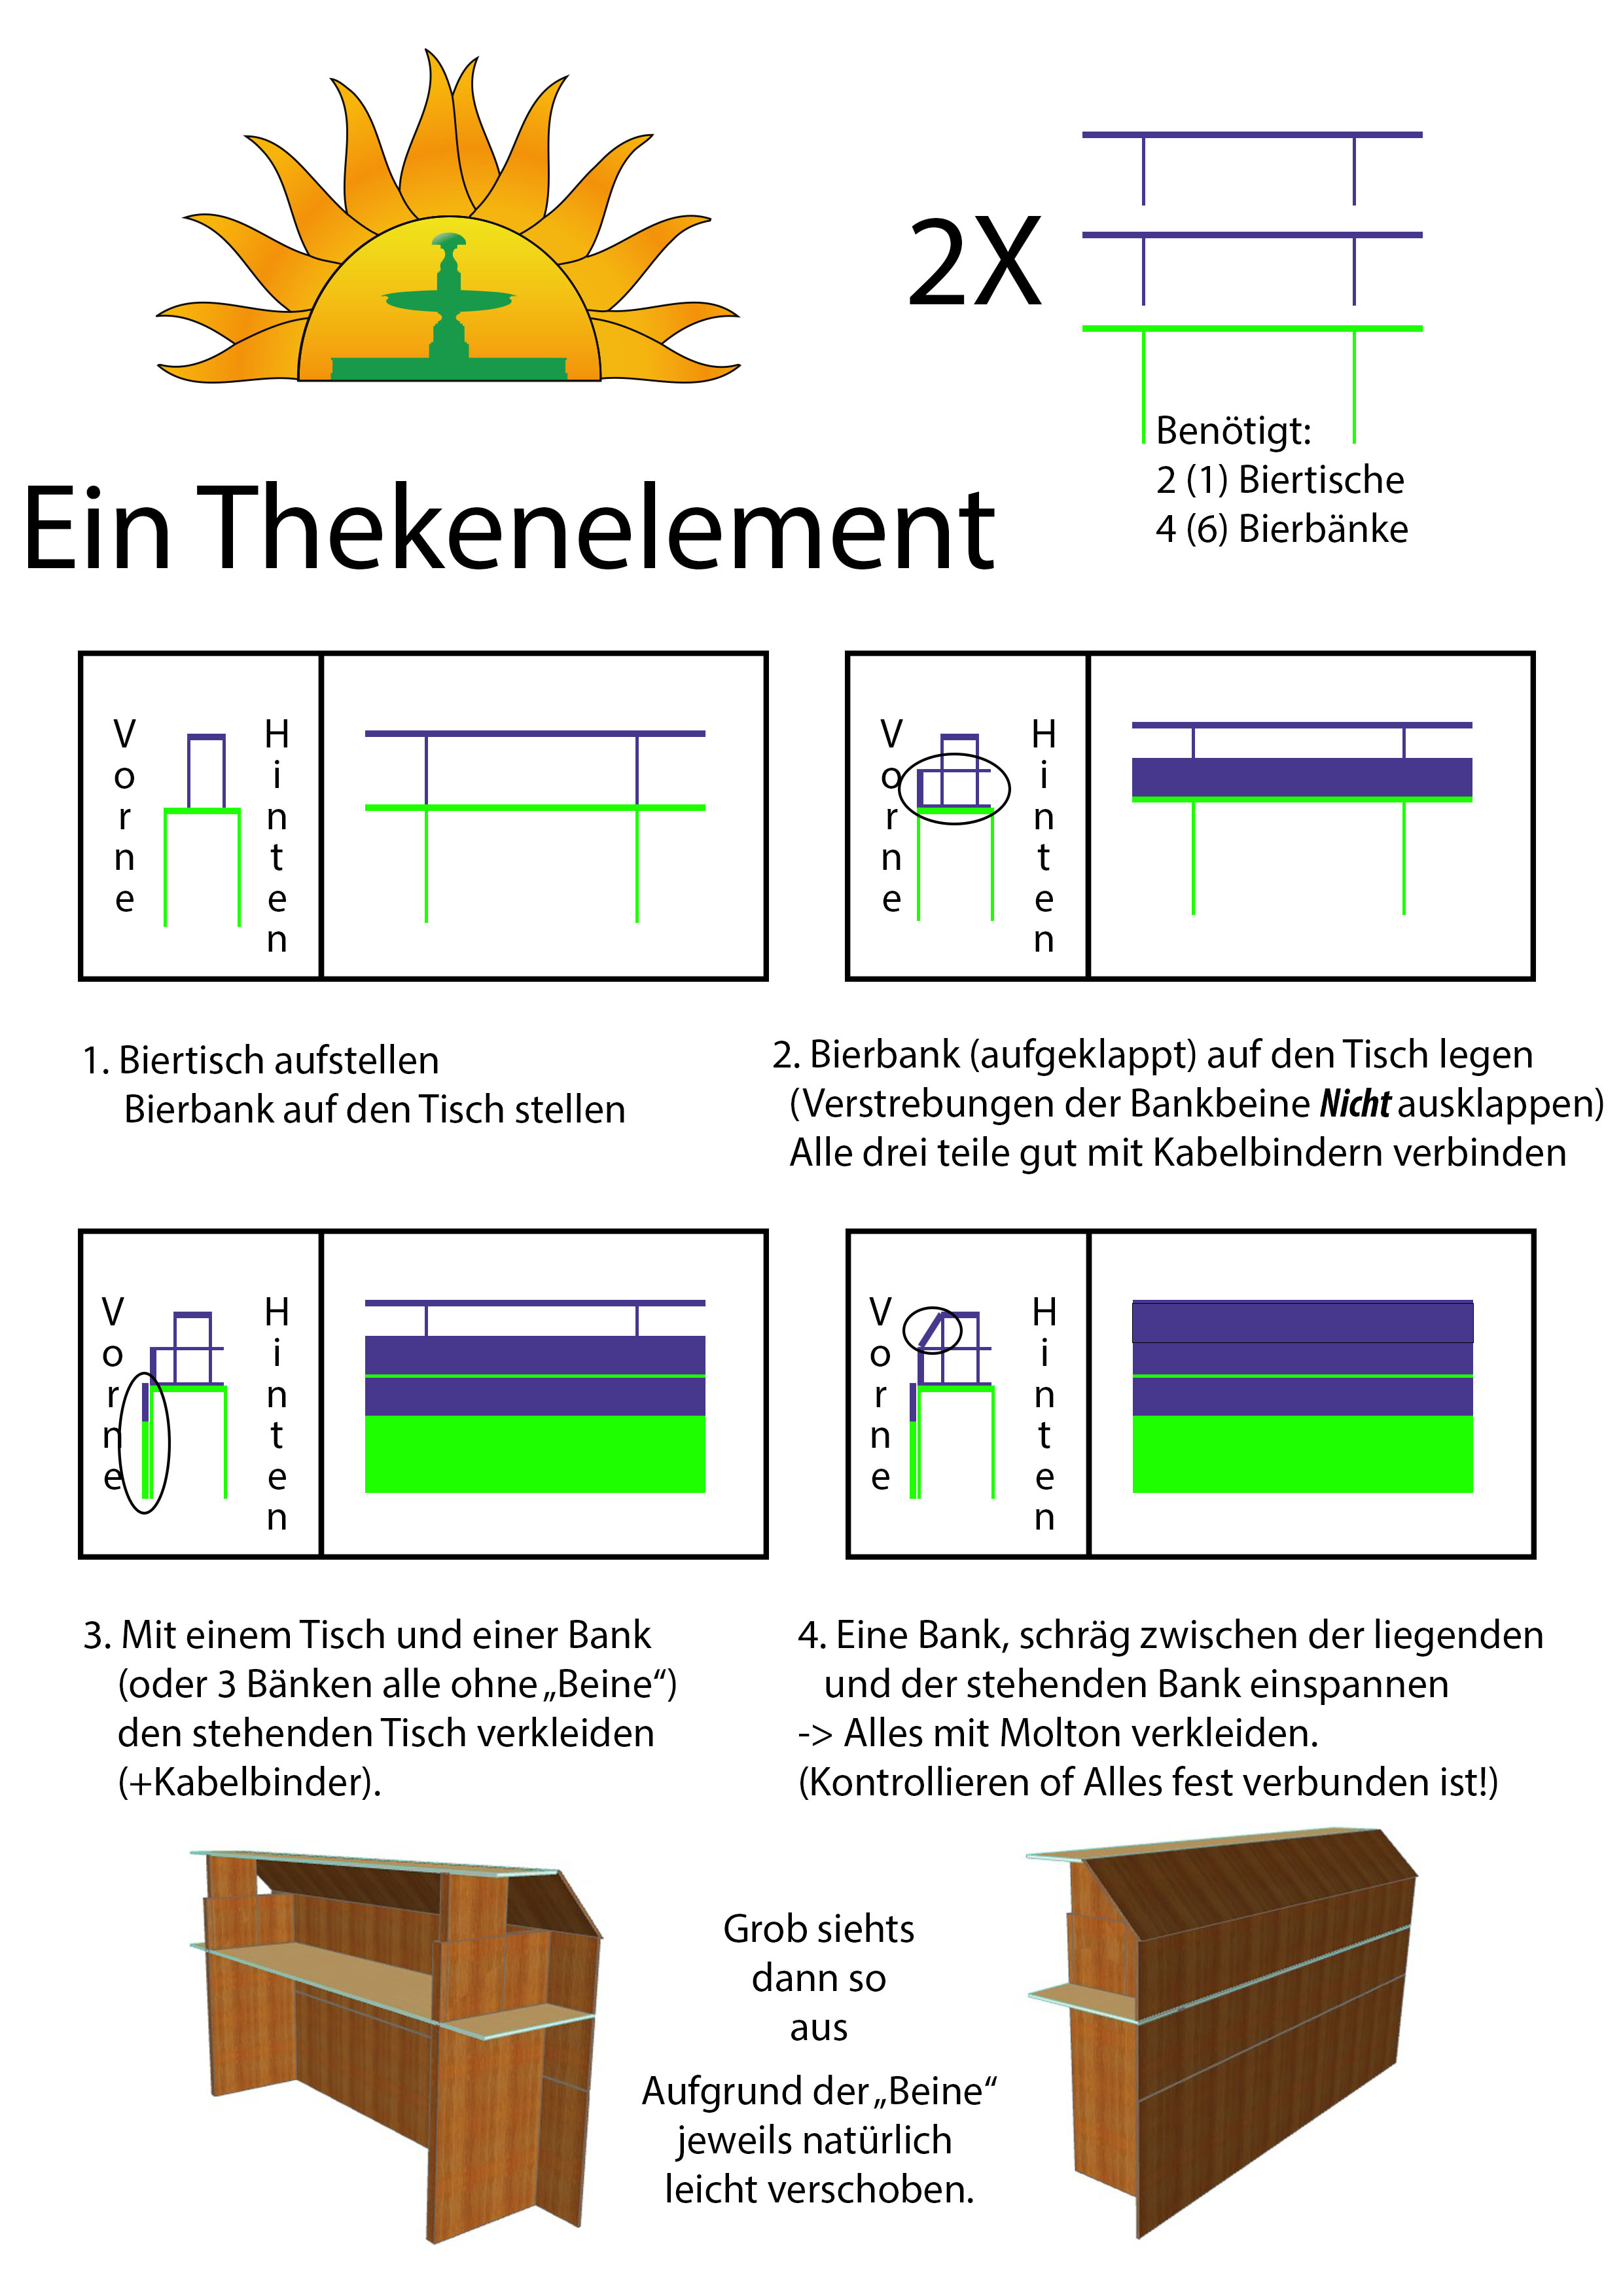
\includegraphics[width=.95\textwidth]{theke.jpg}
%\tiny{
%\begin{figure}[h]
%  \centering
%  \begin{subfigure}[t]{0.45\textwidth}
%    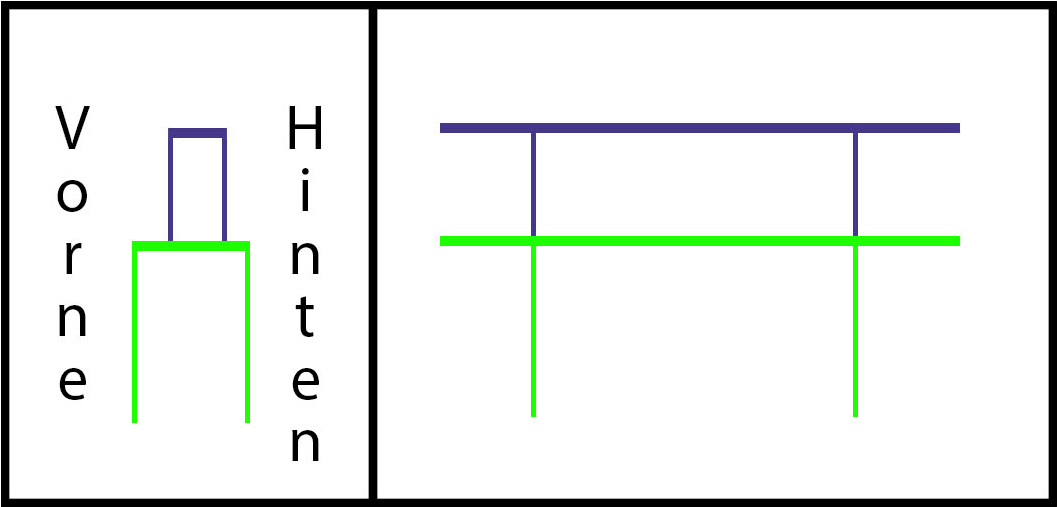
\includegraphics[width=\textwidth]{2d_1.png}
%    \caption{Einen Tisch aufstellen und eine aufgeklappte Bank darauf stellen.}
%  \end{subfigure}
%  \hfill
%  \begin{subfigure}[t]{0.45\textwidth}
%    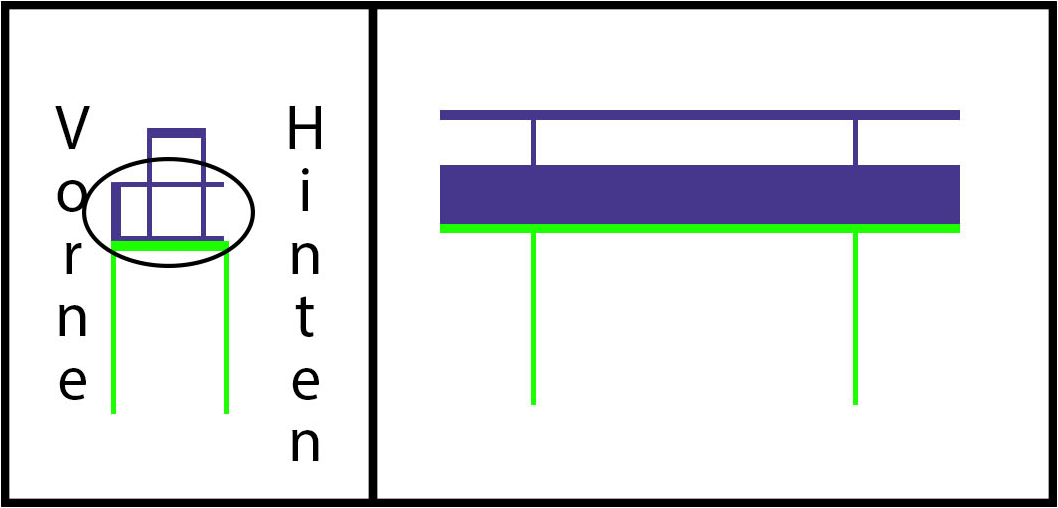
\includegraphics[width=\textwidth]{2d_2.png}
%    \caption{Eine Bank aufklappen, aber die diagonalen Arretierungen eingeklappt lassen. Die Bank senkrecht zum Tisch hinlegen und alle drei Teile mit Kabelbindern befestigen, aber noch nicht ganz festzurren.}
%  \end{subfigure}
%  \centering
%  \begin{subfigure}[t]{0.45\textwidth}
%    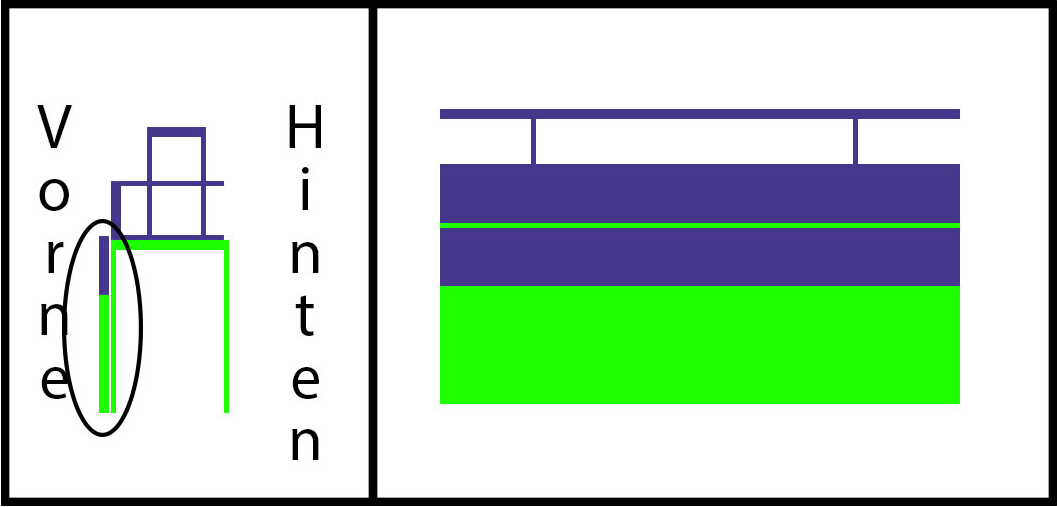
\includegraphics[width=\textwidth]{2d_3.png}
%    \caption{Die Vorderseite mit 1 Tisch und 2 Bänken, oder 3 Bänken verkleiden und mit Kabelbindern verbinden (die Beine jeweils eingeklappt lassen, sonst stehen sie innen über).}
%  \end{subfigure}
%  \hfill
%  \begin{subfigure}[t]{0.45\textwidth}
%    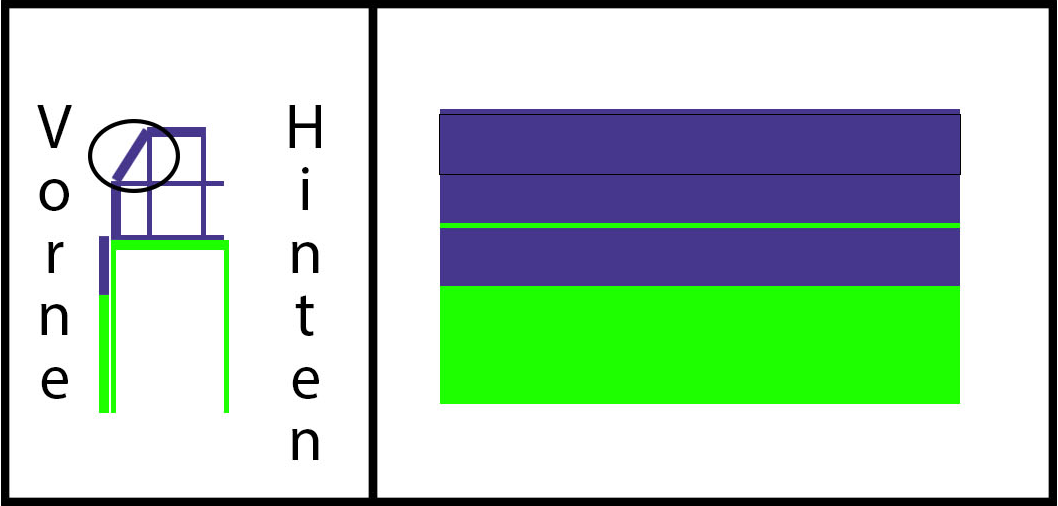
\includegraphics[width=\textwidth]{2d_4.png}
%    \caption{Eine Bank (auch ohne Beine) schräg zwischen der liegenden und der stehenden Bank einspannen und mit Kabelbindern festzurren.}
%  \end{subfigure}
%  \label{theke2d}
%\end{figure}
%\begin{figure}[h]
%  \begin{subfigure}[t]{0.45\textwidth}
%    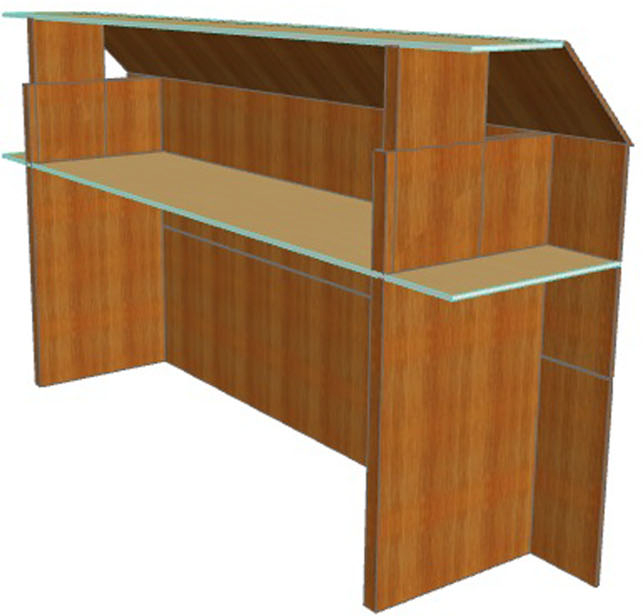
\includegraphics[width=.7\textwidth]{3d_hinten.png}
%  \end{subfigure}
%  \begin{subfigure}[t]{0.45\textwidth}
%    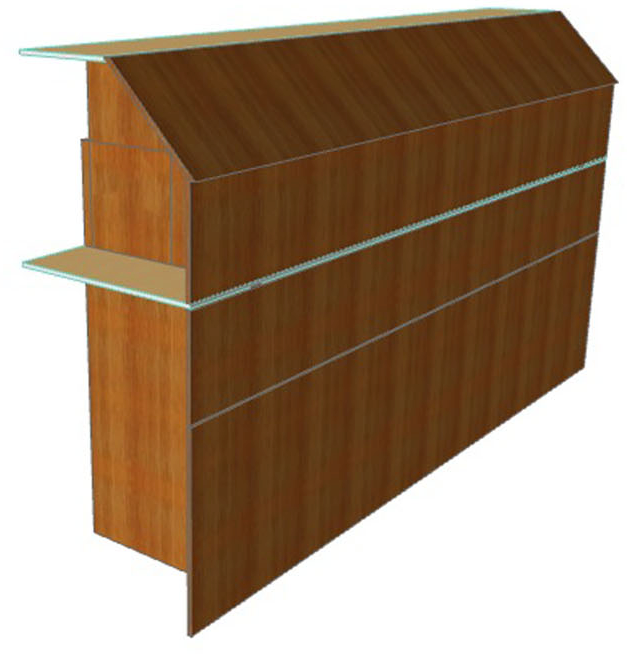
\includegraphics[width=.7\textwidth]{3d_vorne.png}
%  \end{subfigure}
%  \label{theke3d}
%\end{figure}
%}
\subsection{Lageplan}
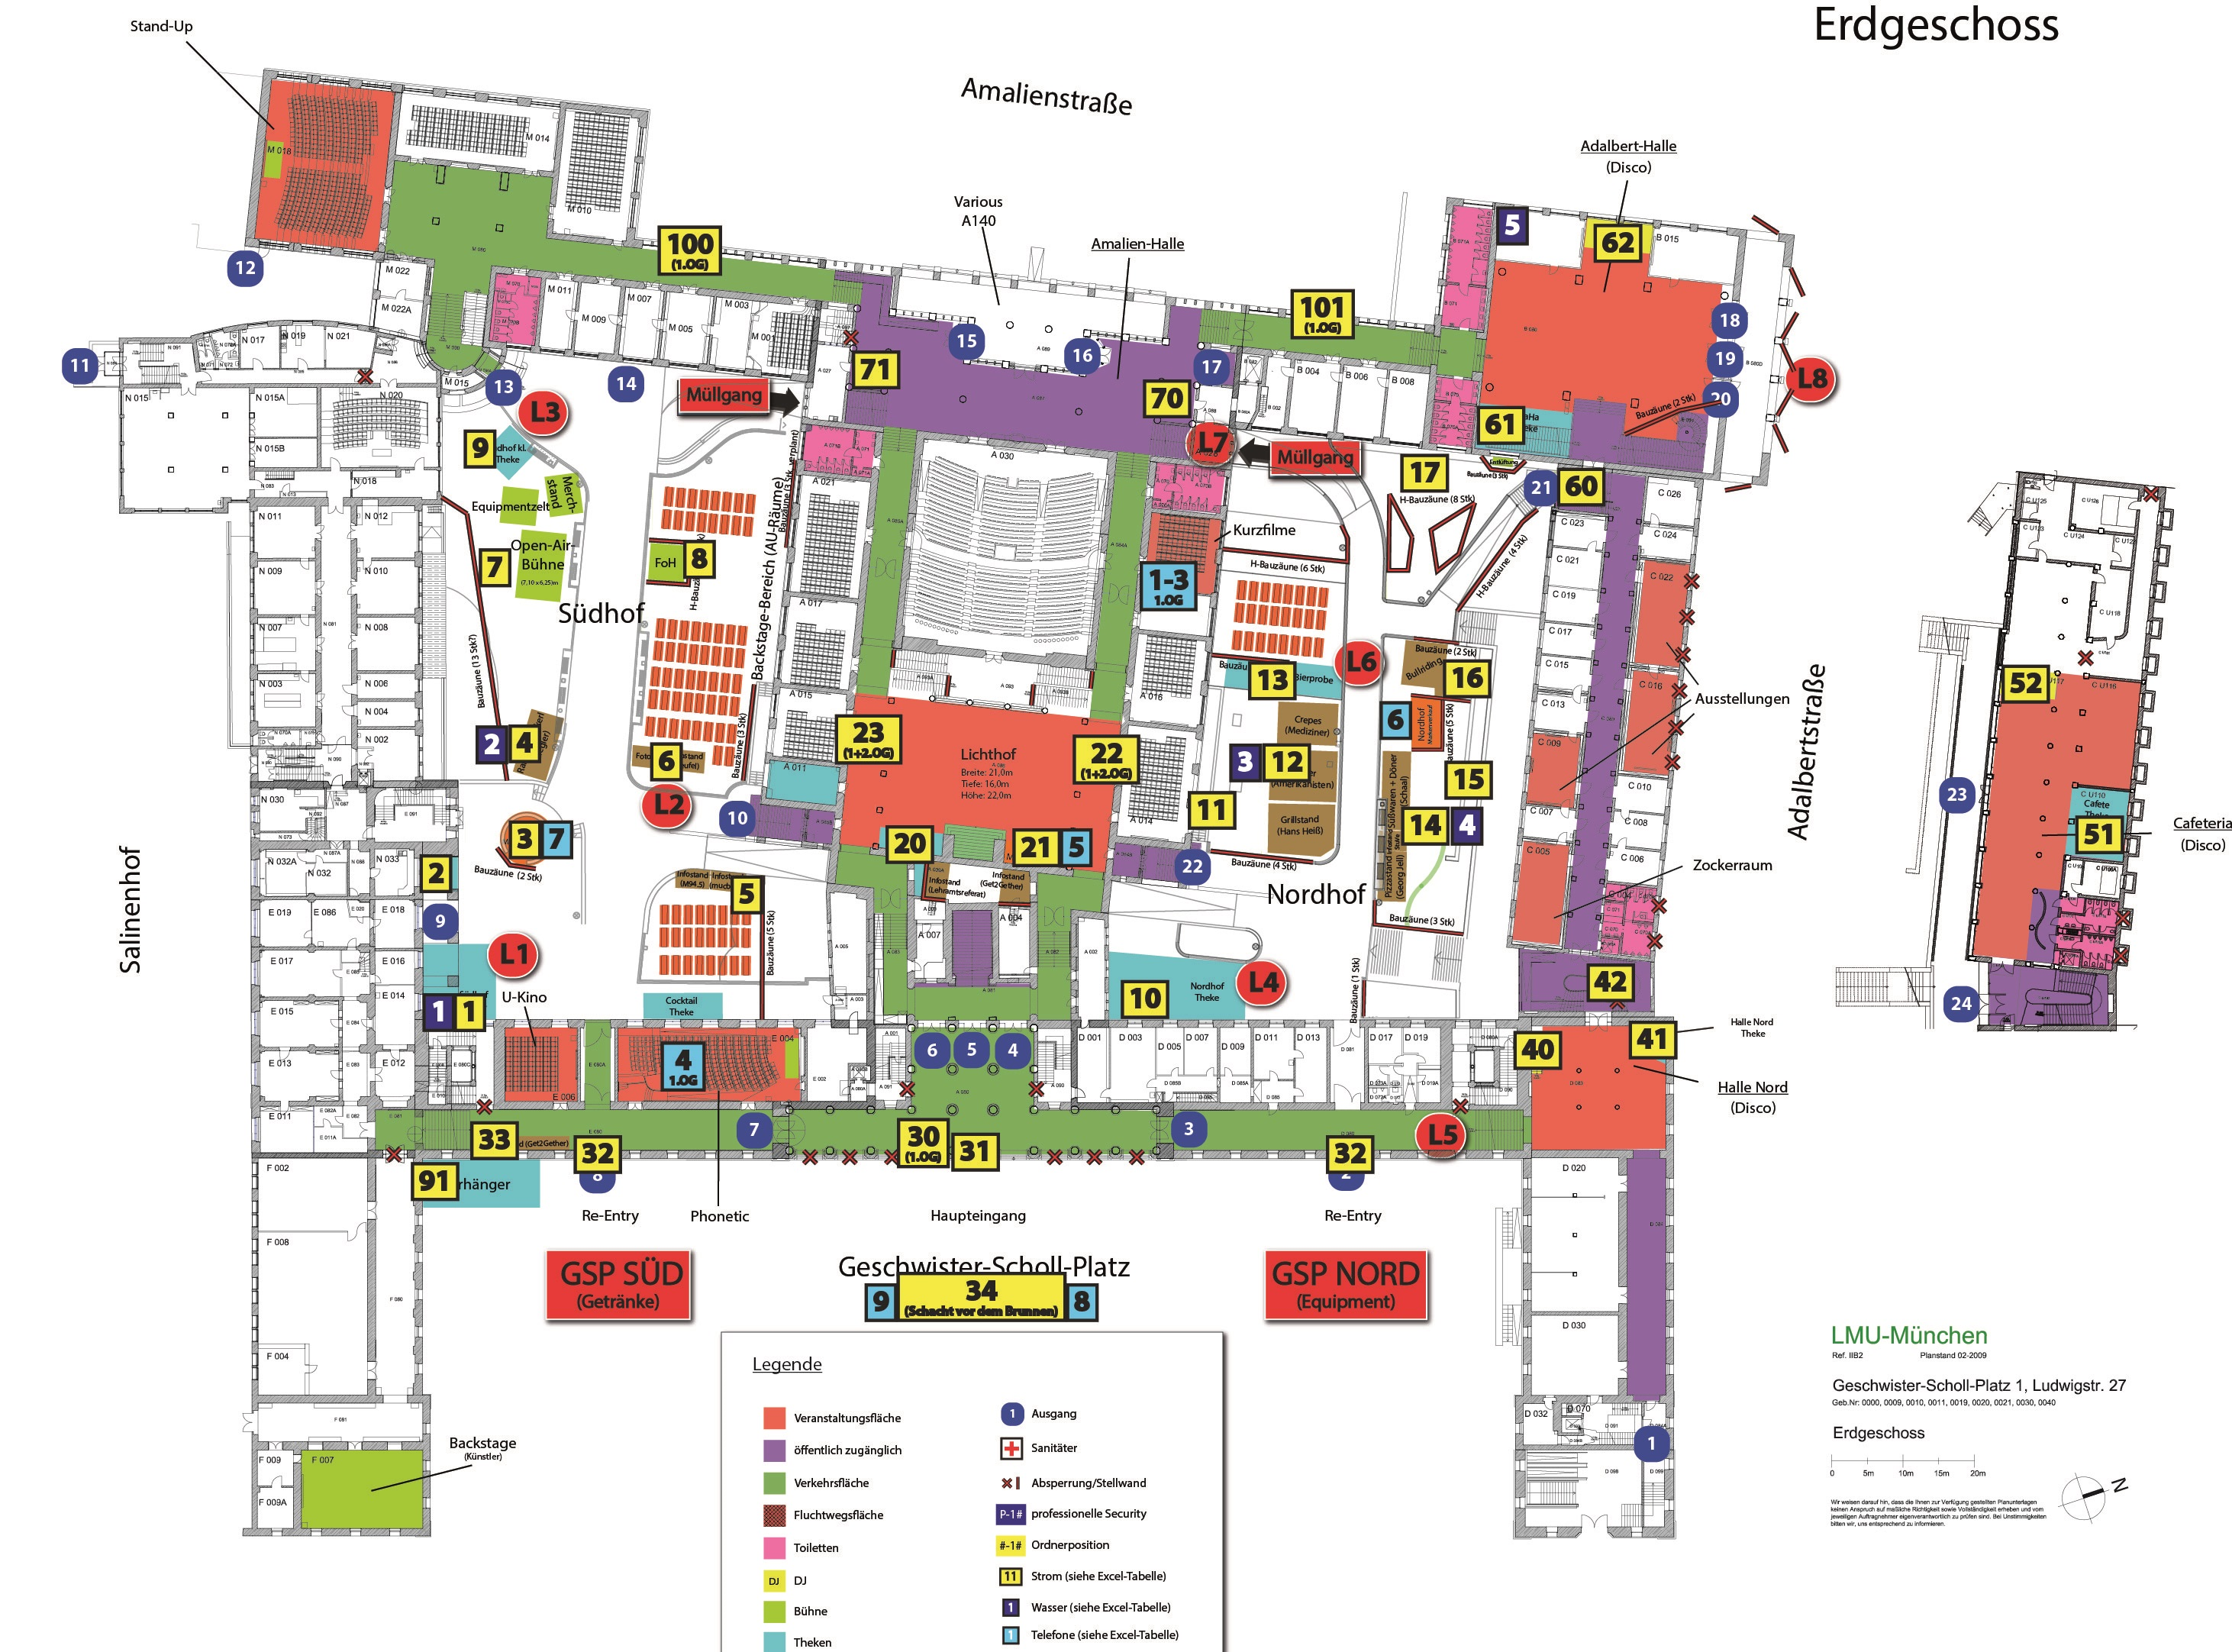
\includegraphics[height=\textwidth, angle=270]{plan.jpg}

\end{document}
